% 
% Annual CCN conference
% Sample LaTeX Two-Page Summary -- Proceedings Format
% based on the prior cognitive science style file

% Original : Ashwin Ram (ashwin@cc.gatech.edu)       04/01/1994
% Modified : Johanna Moore (jmoore@cs.pitt.edu)      03/17/1995
% Modified : David Noelle (noelle@ucsd.edu)          03/15/1996
% Modified : Pat Langley (langley@cs.stanford.edu)   01/26/1997
% Latex2e corrections by Ramin Charles Nakisa        01/28/1997 
% Modified : Tina Eliassi-Rad (eliassi@cs.wisc.edu)  01/31/1998
% Modified : Trisha Yannuzzi (trisha@ircs.upenn.edu) 12/28/1999 (in process)
% Modified : Mary Ellen Foster (M.E.Foster@ed.ac.uk) 12/11/2000
% Modified : Ken Forbus                              01/23/2004
% Modified : Eli M. Silk (esilk@pitt.edu)            05/24/2005
% Modified : Niels Taatgen (taatgen@cmu.edu)        10/24/2006
% Modified : David Noelle (dnoelle@ucmerced.edu)     11/19/2014
% Modified : Konrad Kording (koerding@gmail.com) 2/15/2017

\documentclass[10pt,letterpaper]{article}

\usepackage{ccn}
\usepackage{pslatex}
\usepackage{apacite}
\usepackage{graphicx}

\graphicspath{ {../static/} }

\title{Convolutional neural networks performing a visual search task show attention-like 
limits on accuracy when trained to generalize across multiple search stimuli}
 
\author{{\large \bf David Nicholson (dnicho4@emory.edu)} \\
  A Department, 1234 Example Street\\
A City, State 12345 A country
  \AND {\large \bf Astrid Prinz (AnotherPerson@this.planet.edu)} \\
  A Department, 1234 Example Street\\
A City, State 12345 A country}


\begin{document}

\maketitle


\section{Abstract}
{
\bf
What limits our ability to find what we are looking for in the cluttered noisy world we 
see around us? A now classic form of visual search task has long been used to investigate 
proposed mechanisms of selective attention. In spite of nearly half a century of studies 
using this task, it remains unclear how best to relate different effects found using this 
task to computations that take place in the visual system. A separate thread of research 
has studied the visual system of humans and other primates using convolutional neural 
networks (CNNs) as models. While CNNs have proven quite useful as models of the visual 
system, it also remains unclear the extent to which their behavior mirrors that of 
humans when performing vision-based tasks. Here we investigate whether the accuracy of 
CNNs is affected by the same factors that affect human performance on the classic form of 
visual search task used to investigate attention mechanisms. We first replicate and extend
a previous study which did find that CNNs trained for image classification show human-like
attentional limitations. Then we demonstrate that, by changing how we train the networks, 
these effects can largely be eliminated. Lastly we show that accuracy is impaired when 
single networks are trained to discriminate multiple types of visual search stimuli. Based
on these findings, we suggest that the need to generalize across multiple tasks may be one 
source of limitations on visual search for both CNNs and the primate visual system.
}
\begin{quote}
\small
\textbf{Keywords:} 
attention;visual search
\end{quote}

\section{Introduction}
\subsection{What are the factors that limit visual search?}
What limits our ability to find what we are looking for in the cluttered noisy world we 
see around us? One of the principle tasks that has been used to investigate this question
is a classic form of visual search task, in which subjects view a stimulus on each trial, 
made up of discrete sets of items on a solid-colored background, and report whether a 
target is present among distractors [@wolfeVisualSearch1998]. 
Most studies experimentally manipulate factors such as features of the targets and 
distractors in order to identify the factors limit visual search 
[@ecksteinVisualSearchRetrospective2011; @wolfeFiveFactorsThat2017].
Importantly, it is these factors that *limit* visual search performance that form the 
basis of seminal theories of selective visual attention, although authors differ in the 
extent to which they identify limitations on visual search as synonymous with selective 
attention. To remain neutral, we will use the term "capacity limitations". 
As we review briefly below for context, there are essentially two competing proposed 
sources of capacity limitations [@palmerSignalDetectionEvidence2011]. 
The results supporting both remain unreconciled, in spite of nearly half a century of 
studies based on this task. The core question is: to 
what extent can limitations on visual search be attributed to an attention-like 
computation, e.g. binding features into items, and to what extent can those limitations be 
attributed to other computations, e.g. a decision-making process subject to  
noisy internal representations?
To foreshadow our approach below, we suggest that another way of posing this question is 
to ask: if some algorithm could produce a statistical model capable of learning from data 
to classify visual search stimuli as "target present" or "target absent" with high 
accuracy, would the accuracy still be subject to some ceiling, due simply to the 
constraints of the task? This way of posing the question bears some similarity to a 
well-established framework in vision research known as ideal observer analsyis 
[@geislerIdealObserverAnalysis2003]. However, few ideal observer models have take the 
form of "pixel-in, behavior-out", and the few that have do not generalize to many 
different types of visual search stimuli, so their predictive power is limited 
[@geislerModelsOvertAttention2011].

Before we discuss how to address this gap in models, we briefly review the two competing 
proposed sources of capacity limitations, and describe how they depend in part on the 
way the visual search task is performed. Adopting the terms of other researchers, we will 
call the first family "attention-limited", and the second "noise-limited" 
[@palmerSignalDetectionEvidence2011]. Both attention-limited and noise-limited models 
depend on what are known as *set-size effects* seem when using visual search stimuli, 
which we will define in terms of how the visual search task is carried out. 
Attention-limited models posit two-stage theories of visual processing, a first 
*preattentive* stage which can process single features, such as color or orientation, 
in parallel, and a second *attentive* stage that binds features to objects that processes 
serially, which results in a bottleneck [@treismanFeatureintegrationAttention1980; 
@wolfeGuidedSearchRevised1994]. Evidence for this theory came from visual search 
experiments where subjects were shown stimuli until responding, and their reaction time 
was measured. Plotting reaction time as a function of set size revealed 
lines whose slope were near zero when a single feature distinguished the target from 
distractors (e.g., "red" v. "green"). The slope of reaction time v. set size increased 
sharply, though, when distinguishing the target from distractors required finding a 
conjunction of features (such as "red vertical" v. "red horizontal or green vertical"). 
This sort of set size effect has been replicated hundreds of times, although it remains 
unclear why some search stimuli seem to be processed effectively in parallel while others 
face a bottleneck [@wolfeWhatCanMillion1998; @wolfeFiveFactorsThat2017].
The second family of capacity limitations can be conceived of as completely parallel but 
noisy processing. These models arose in large part in reaction 
to the way the visual search task was carried out when investigating
serial mechanisms. Early studies that measured reaction times left several factors 
uncontrolled, such as target-distractor similarity [@duncanVisualSearchStimulus1989], 
drops in acuity outside the fovea, eye movements, and effects resulting from visual 
crowding [@bergenRapidDiscriminationVisual1983; @ecksteinLowerVisualSearch1998]. 
Hence researchers designed versions of the visual search task that controlled for such 
factors [@palmerPsychophysicsVisualSearch2000]. Crucially, they showed subjects the 
stimulus only briefly, to prevent eye movements, and measured accuracy instead of reaction
time. Computational models of parallel mechanisms succesfully explained results from 
single feature and conjunction search stimuli. These models borrowed ideas from signal 
detection theory that psychophysicists often employ, where sensory representations are
imagined as distributions, and decisions are seen as thresholds on those distributions.
What both attention-limited and noise-limited models have in common is that they are 
both highly abstracted models of the visual system, in which low-level features pass 
through a hierarchy until reaching a final stage consisting of a simple decision rule.

\subsection{CNNs as models of the visual system?}
Similarly, the architecture of convolutional neural networks (CNNs) now routinely used for
computer vision tasks represents a highly abstracted view of the visual system.
Many researchers have drawn parallels between the architecture of CNNs and the 
architecture of the visual system in the brain [@kriegeskorteDeepNeuralNetworks2015], 
in particular in humans and other primates where this system has been most thoroughly 
studied. Like CNNs, the visual system has a hierarchical structure, and is thought to 
function in part by performing transformations at each level of this hierarchy so that 
high-dimensional, low-level features are mapped into low-dimensional abstract 
representations. Several recent studies in the realm of cognitive neuroscience 
have measured representations in more directly tested the similarities between CNNs and 
the visual system, by comparing representations in both [@khaligh-razaviDeepSupervisedNot2014; @yaminsPerformanceoptimizedHierarchicalModels2014; @yaminsUsingGoaldrivenDeep2016]. Representations 
can be easily extracted from CNNs because they are "transparent box" models--i.e. we have 
access to the "activity" of the individual units from which these models are built when 
we "show" the CNNs a stimulus.
A natural question to ask, for someone interested in visual search and models of the visual 
system, is how CNNs perform this task. If CNNs are excellent models of the visual system, 
one might expect them to be subject to the same limitations on visual search. Alternatively, 
if CNNs are simply function approximators, one might expect that they would be able to 
very easily learn to map the exclusive-or function of "target present or target absent", 
especially when targets and distractors are easily discriminated by single feature 
dimensions such as color. While there have been previous studies of neural networks 
performing visual search tasks, we are aware of only one that employed architectures 
which have been used in studies of the visual system referenced above.

\begin{figure}[ht]
\begin{center}
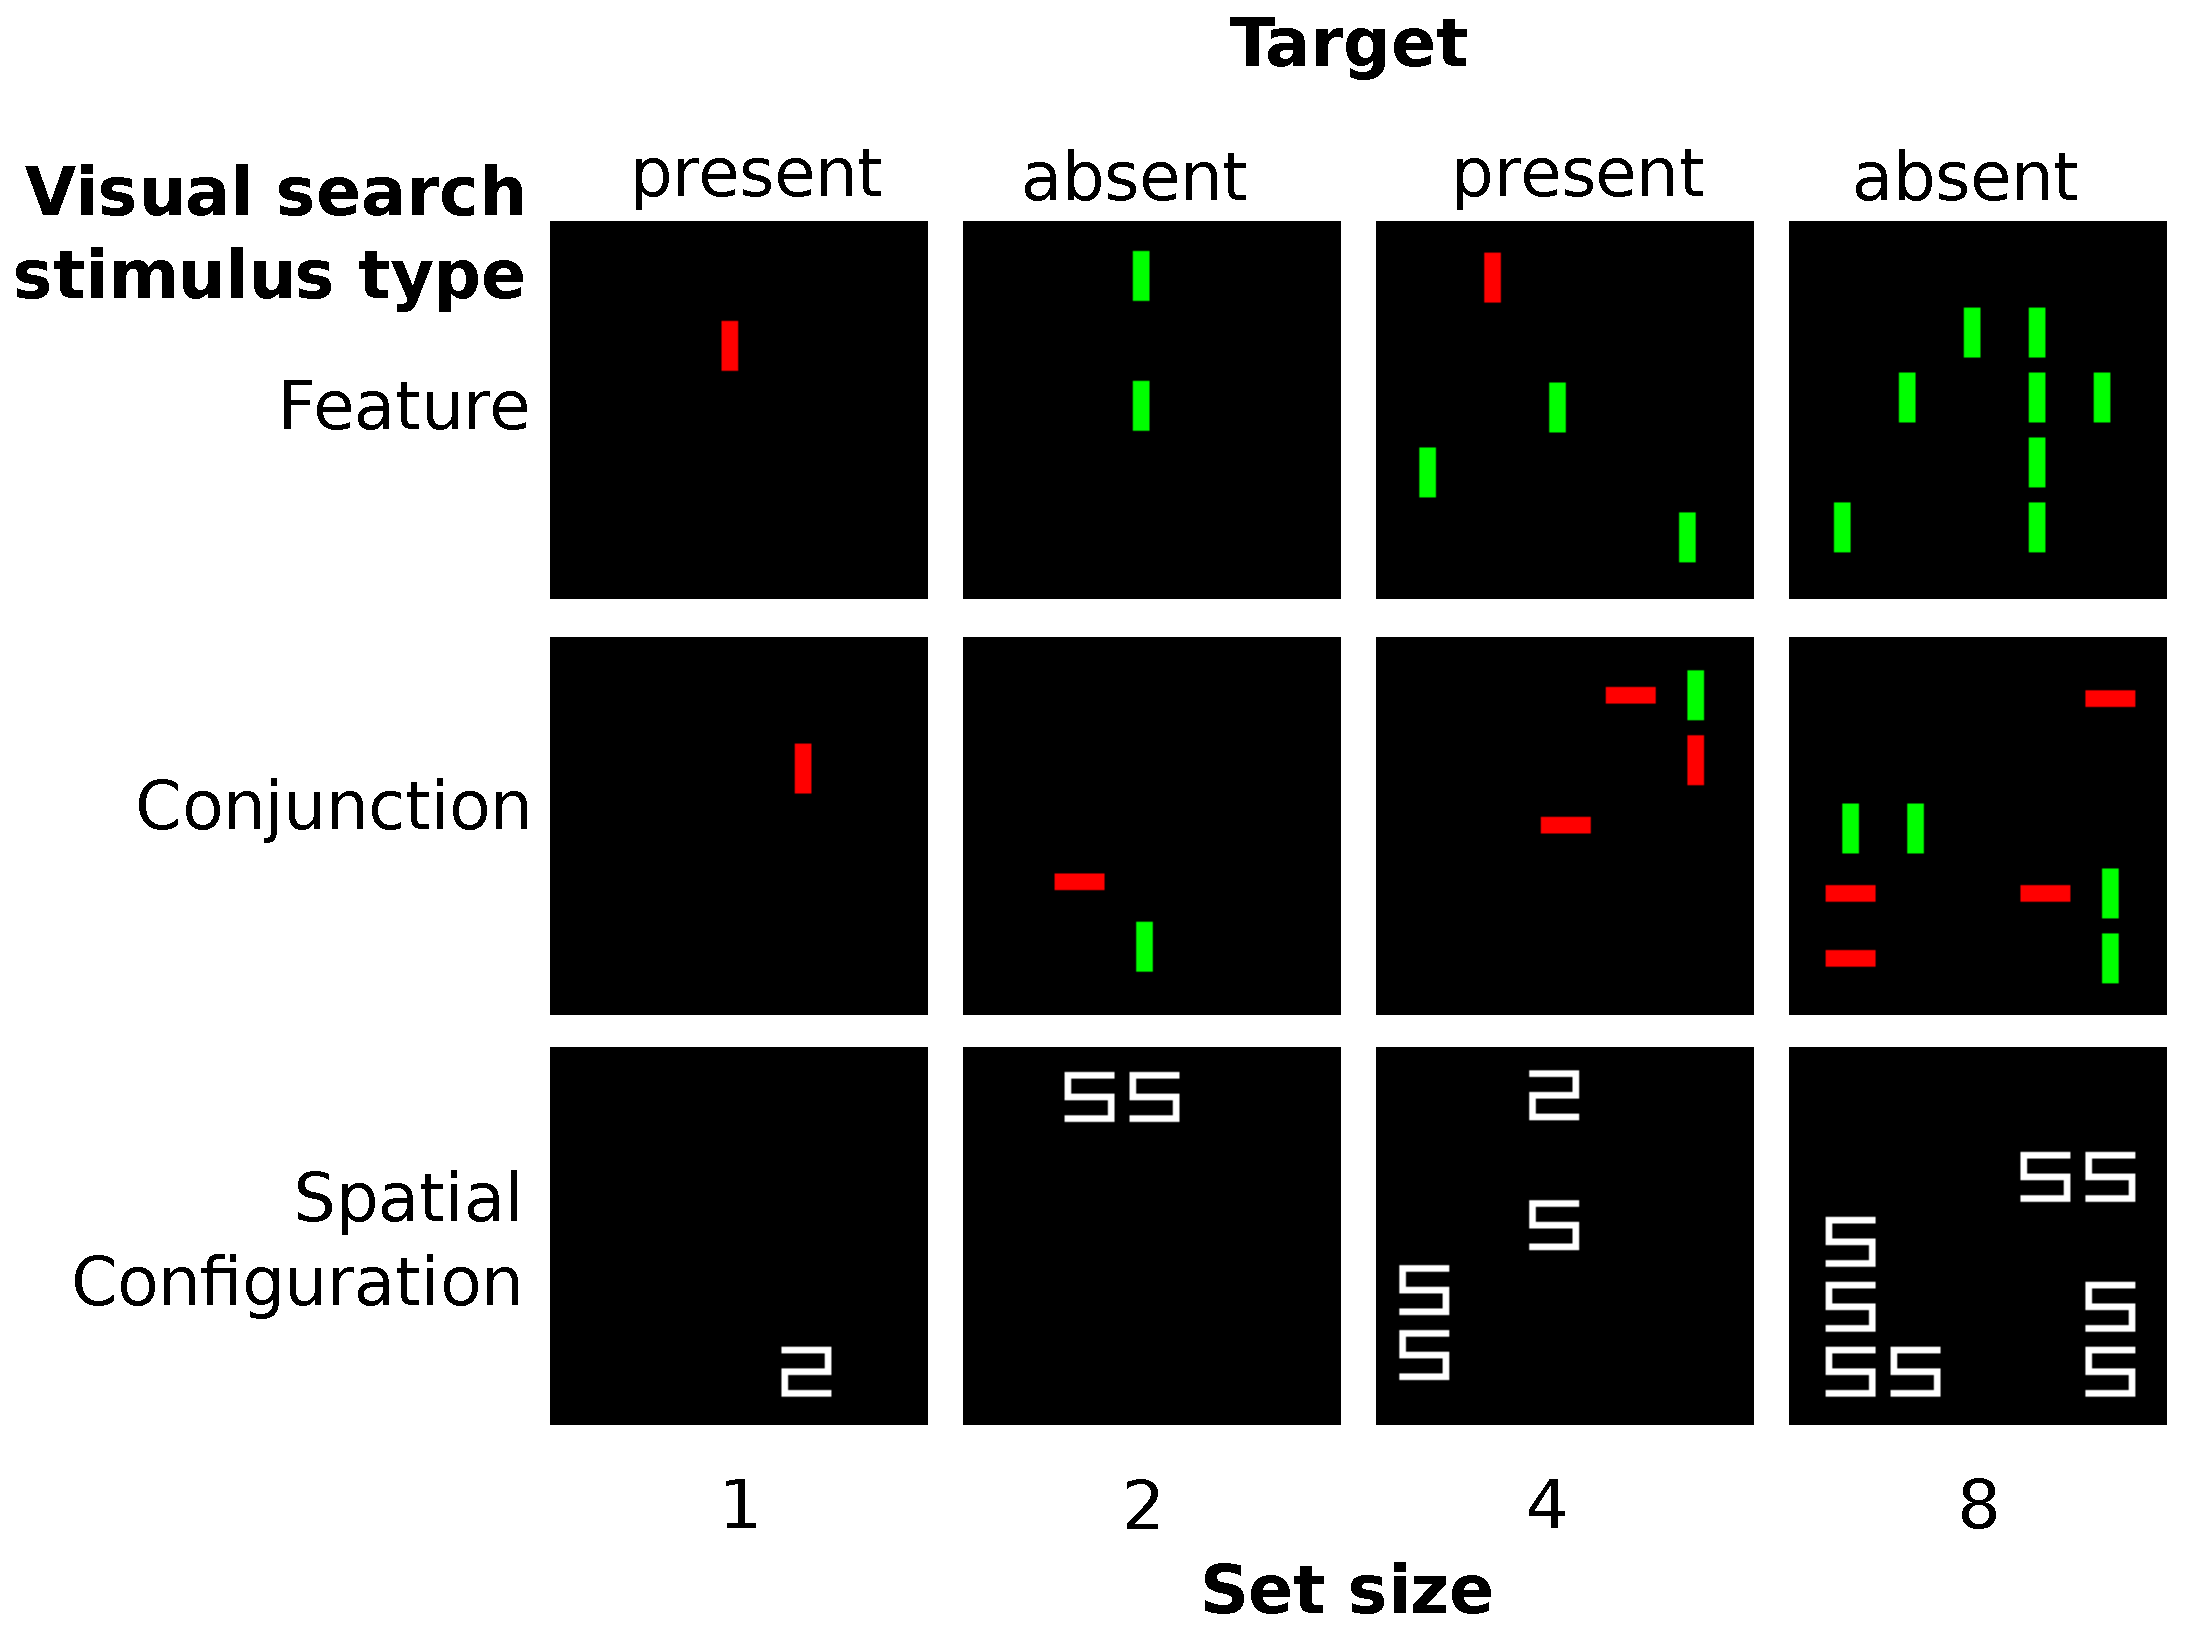
\includegraphics[width=\columnwidth]{fig1/fig1.eps}
\end{center}
\caption{A classic form of visual search task.} 
\label{sample-figure}
\end{figure}



\section{Results}

\subsection{CNNs trained for image classification show set size effects}

\begin{figure}[ht]
\begin{center}
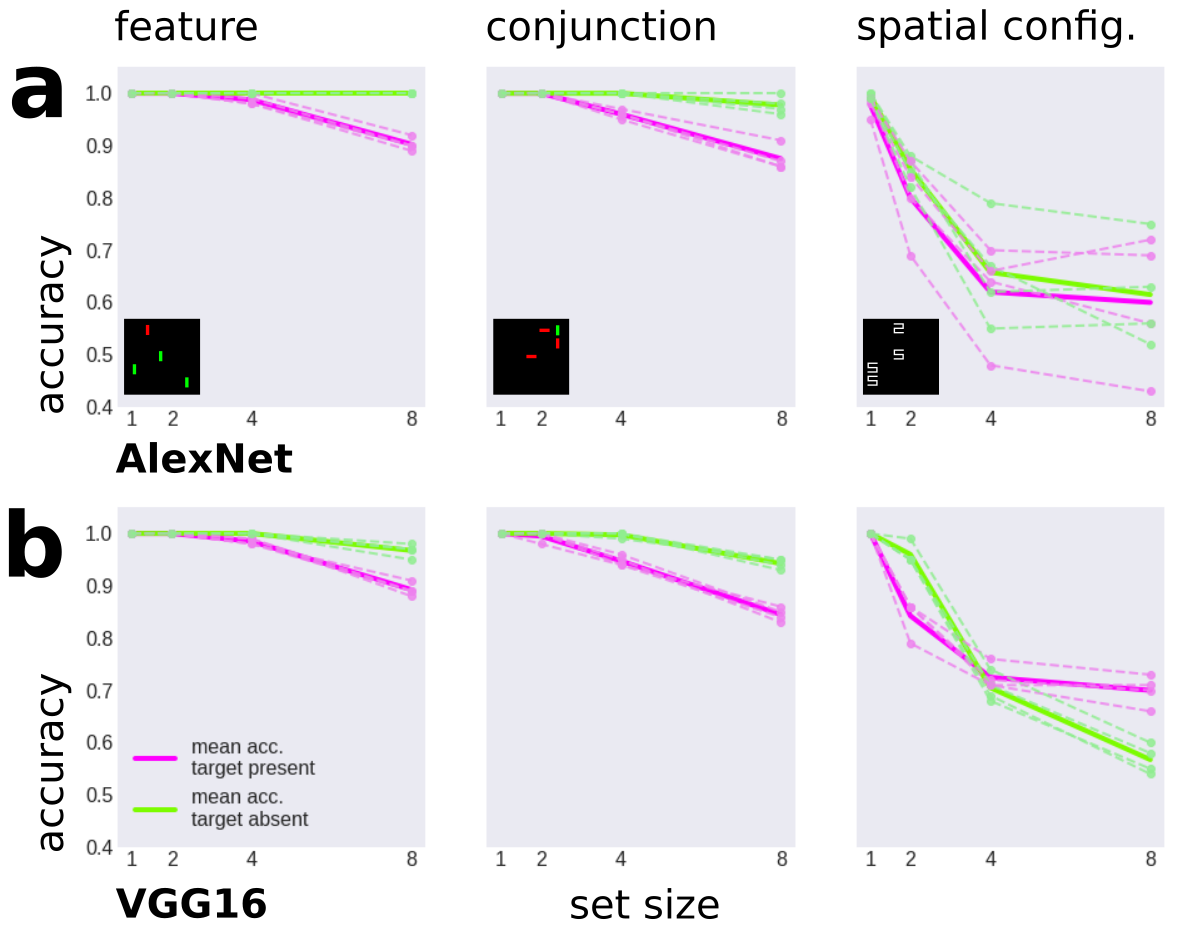
\includegraphics[width=\columnwidth]{fig2/fig2.png}
\end{center}
\caption{CNNs trained for image classification show set size effects.} 
\label{sample-figure}
\end{figure}


\subsection{Changing hyperparameters and balancing the dataset largely 
eliminates set size effects}

Because we defined set size with effects in terms of accuracy, it could 
be the case that our results do not arise because of a similarity between 
how CNNs and brains process images. Instead they could be an artifact of 
how we trained networks. As discussed below, we see this as a general issue 
for studies that compare cognitive science and artificial intelligence, and 
so here we report results that might otherwise be considered methodological 
troubleshooting.
To determine whether our results were an artifact of training, we considered aspects of 
training that can impair accuracy: the amount of training data, the hyperparameters 
used to train the network, and the statistics of the dataset. As shown in 
figure two, we found that all three factors contributed to the effect we saw.
We generated learning curves where we plotted accuracy on the training and 
test set as a function of the training set size. These learning curves revealed 
that the original size we chose for the training set was far from where 
accuracy on training and test set converged. This result indicates that the 
network can improve accuracy with increased training data. To gain insight 
about how accuracy depended on the learning rate, a key hyperparameter, and 
the balance of the data set, we plotted accuracy on the training set 
\emph{separately for each set size in the visual search stimuli}. As shown in 
figure 2b, these plots revealed (1) that accuracy had not yet reached some asymptotic 
value, and (2) that there was an inverse relationship between the set size of 
a visual search stimulus and the rate that its accuracy increased.
To test whether we could improve the learning rate, we used random search, and 
did find we were able to improve accuracy and decrease training time by 
abandoning the fine-tuning approach and instead using a typical learning rate 
on the fully-connected layers (and simply freezing the pre-trained weights in other layers). 

Use standard APA citation format. Citations within the text should
include the author's last name and year. If the authors' names are
included in the sentence, place only the year in parentheses, as in
\citeA{NewellSimon1972a}, but otherwise place the entire reference in
parentheses with the authors and year separated by a comma
\cite{NewellSimon1972a}. List multiple references alphabetically and
separate them by semicolons
\cite{ChalnickBillman1988a,NewellSimon1972a}. Use the
``et~al.'' construction only after listing all the authors to a
publication in an earlier reference and for citations with four or
more authors.

\section{Discussion}

\subsection{Implications for comparative studies of neuroscience and 
artificial intelligence}
- problem for any 

- e.g. Bengio study of gestalt fx

\subsection{Implications for the study of attention in the brain}
- if the task is possible to perform perfectly, who needs attention?
- brain optimized for something else besides classifying static images
- in this sense, consistent with findings that recurrent

\subsection{Footnotes}

Indicate footnotes with a number\footnote{Sample of the first
footnote.} in the text. Place the footnotes in 9~point type at the
bottom of the column on which they appear. Precede the footnote block
with a horizontal rule.\footnote{Sample of the second footnote.}


\subsection{Tables}

Number tables consecutively. Place the table number and title (in
10~point) above the table with one line space above the caption and
one line space below it, as in Table~\ref{sample-table}. You may float
tables to the top or bottom of a column, or set wide tables across
both columns.

\begin{table}[!ht]
\begin{center} 
\caption{Sample table title.} 
\label{sample-table} 
\vskip 0.12in
\begin{tabular}{ll} 
\hline
Error type    &  Example \\
\hline
Take smaller        &   63 - 44 = 21 \\
Always borrow~~~~   &   96 - 42 = 34 \\
0 - N = N           &   70 - 47 = 37 \\
0 - N = 0           &   70 - 47 = 30 \\
\hline
\end{tabular} 
\end{center} 
\end{table}


\subsection{Figures}

Make sure that the artwork can be printed well (e.g. dark colors) and that 
the figures make understanding the paper easy.
 Number figures sequentially, placing the figure
number and caption, in 10~point, after the figure with one line space
above the caption and one line space below it, as in
Figure~\ref{sample-figure}. If necessary, leave extra white space at
the bottom of the page to avoid splitting the figure and figure
caption. You may float figures to the top or bottom of a column, or
set wide figures across both columns.

\begin{figure}[ht]
\begin{center}
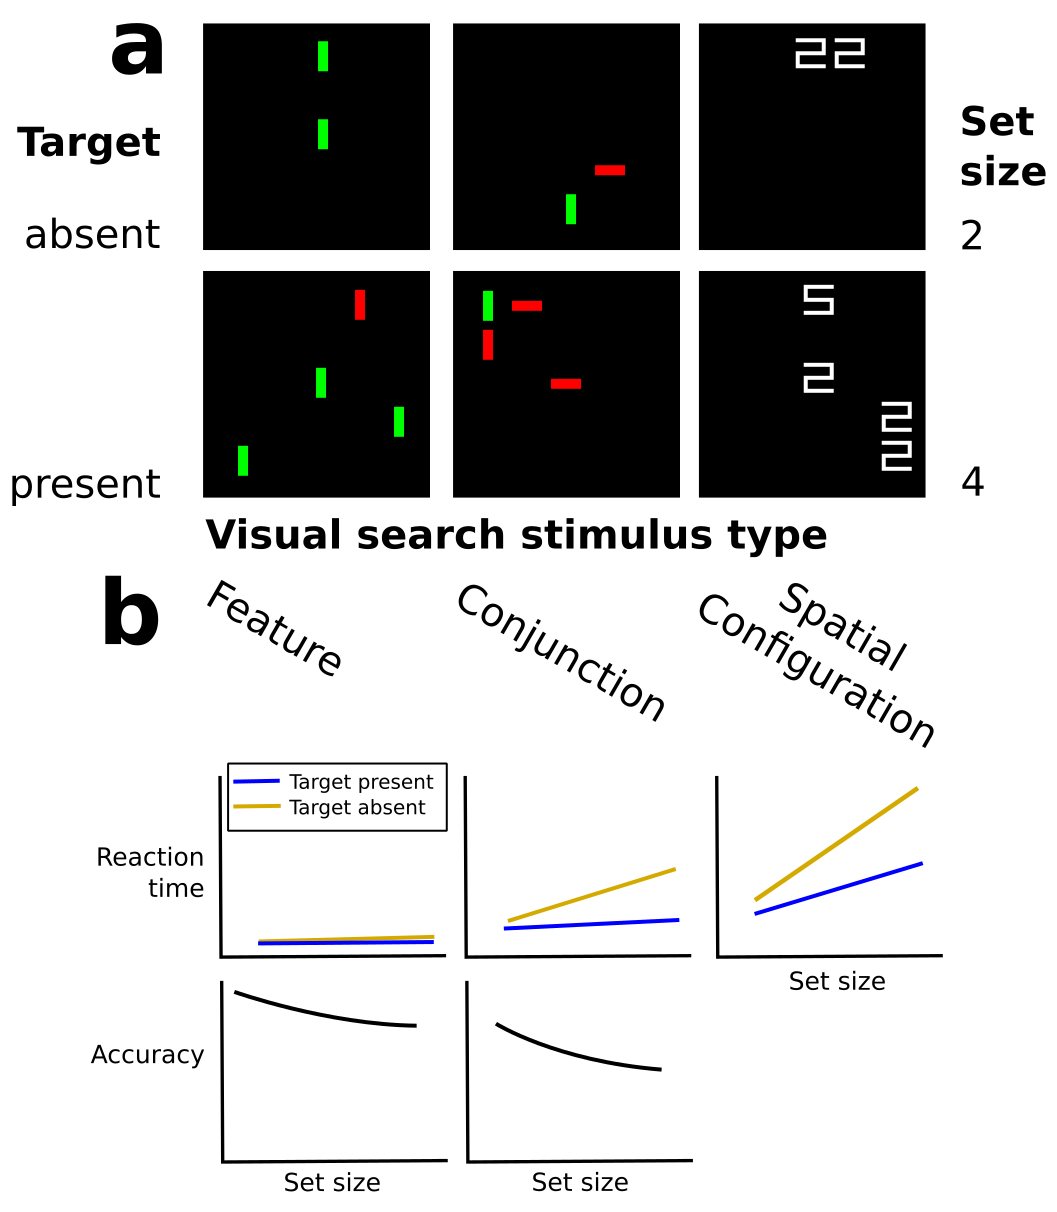
\includegraphics{fig1}
\end{center}
\caption{This is a figure.} 
\label{sample-figure}
\end{figure}


\section{Acknowledgments}

Place acknowledgments (including funding information) in a section at
the end of the paper.


\section{References Instructions}

Follow the APA Publication Manual for citation format, both within the
text and in the reference list, with the following exceptions: (a) do
not cite the page numbers of any book, including chapters in edited
volumes; (b) use the same format for unpublished references as for
published ones. Alphabetize references by the surnames of the authors,
with single author entries preceding multiple author entries. Order
references by the same authors by the year of publication, with the
earliest first.

Use a first level section heading, ``{\bf References}'', as shown
below. Use a hanging indent style, with the first line of the
reference flush against the left margin and subsequent lines indented
by 1/8~inch. Below are example references for a conference paper, book
chapter, journal article, dissertation, book, technical report, and
edited volume, respectively.

\nocite{ChalnickBillman1988a}
\nocite{Feigenbaum1963a}
\nocite{Hill1983a}
\nocite{OhlssonLangley1985a}
% \nocite{Lewis1978a}
\nocite{Matlock2001}
\nocite{NewellSimon1972a}
\nocite{ShragerLangley1990a}


\bibliographystyle{apacite}

\setlength{\bibleftmargin}{.125in}
\setlength{\bibindent}{-\bibleftmargin}

\bibliography{ccn_style}


\end{document}
